%
% Documento: Metodologia
%
\chapter{Metodologia}
\label{chap:Metod}
Para a realização deste trabalho, primeiramente fez-se um estudo das estratégias de controle de formação de robôs móveis, das possibilidades %viabilidade 
de implementação dessas estratégias na plataforma a ser utilizada (no caso, o \emph{Lego Mindstorms\textregistered}) e da viabilidade de modelar e implementar o sistema como um sistema distribuído descentralizado. Onde não tem-se um mestre definido, apenas uma sociedade de robôs que conforme precisam executar uma tarefa, vão recrutando e formando uma frota. 

Após realizados os estudos, concluiu-se que, apesar de viável como pode ser visto no capítulo \ref{chap:trabalhosRelacionados}, a implementação de um sistema distribuído descentralizado seria muito complexo para ser abordado no período proposto para a realização deste trabalho, que tem como objetivo principal o estudo de estratégias de controle de formação de múltiplos robôs móveis. Para tanto, foi adotada uma estrutura de rede centralizada denominada 'Mestre/Escravo', utilizando a comunicação via \emph{Bluetooth}, a qual a própria plataforma e linguagem (\emph{NXT}) dão suporte. 

%Além disso, será feito um controle em cascata, onde a saída de um módulo de controle  utilizado para modularizar o problema e assim, tornar mais simples a implementação e o entendimento do mesmo. %Ponto?
%Além de facilitar na validação do sistema, que foi implementado da malha mais interna à malha mais externa, sendo testado e validado módulo à módulo de controle, bem como suas integrações.  %Para facilitar a implementação, a modelagem foi implementada em módulos de controle, com o intuito de simplificar o entendimento e a validação do sistema. A implementação foi feita da malha mais interna à malha mais externa, sendo testado e validado módulo à modulo de controle, bem como suas integrações.

Existem diversas maneiras de se implementar um sistema como este, tanto do ponto de vista do sistema distribuído e sua rede de comunicação, quanto do ponto de vista de controle e realimentação das malhas. Foram escolhidas duas estratégias diferentes de formação de múltiplos robôs móveis e fez-se então, duas abordagens distintas. Uma delas que atende apenas à um dos problemas e uma outra abordagem mais genérica que pode ser adaptada para a resolução de ambos os problemas. 

Para estabelecer o modelo matemático do problema, foi considerado o modelo de robô mostrado na \autoref{fig:robo}, que consistem em um modelo não holonômico, onde tem-se duas rodas unidirecionais e uma roda orientável. Para definição do modelo matemático levou-se em consideração que os \emph{encoders} seriam utilizados para odometria e então, foram definidas as restrições da modelagem matemática do problema que, desconsidera problemas como: saturação do atuador, derrapagem das rodas, os erros de medição dos \emph{encoders} bem como, as limitações da plataforma. %Tendo em vista um levantamento das dificuldades que surgiram somente na implementação do sistema no mundo real, foi-se adaptando as soluções para o problema e o problema, de forma a viabilizar a correção de erros de sensoriamento que se acumulam a cada iteração.

\begin{figure}[!htb]
	\centering
	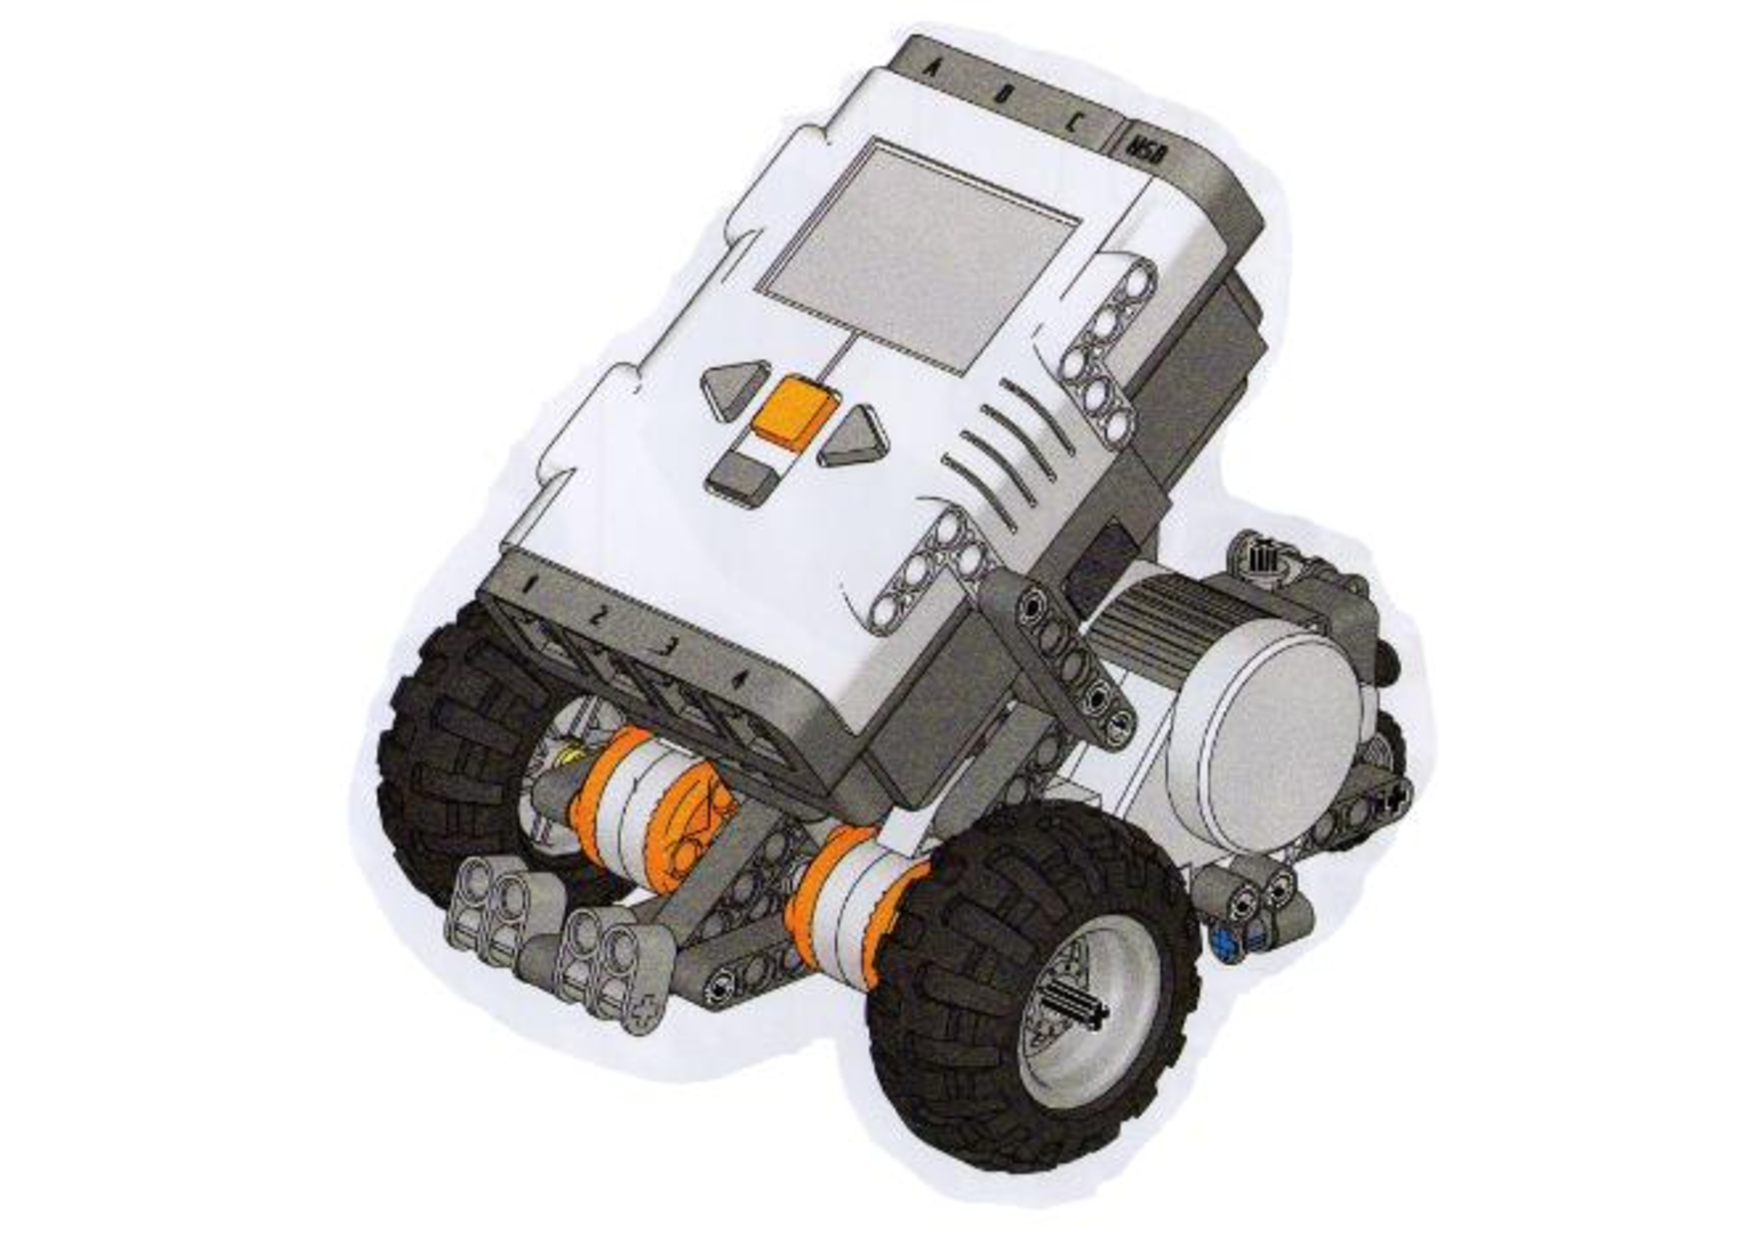
\includegraphics[width=10cm]{./04-figuras/robo}
	\caption{Modelo do Robô}
	\label{fig:robo}
\end{figure}

Após feita a modelagem do problema, foram feitas as implementações e os testes, onde seria possível observar se a odometria feita seria suficiente para alimentar o sistema com precisão e tornar a solução viável. Levando-se em consideração que para tanto foram utilizados os \emph{encoders} óticos acoplados aos motores do \emph{kit Lego Mindstorms\textregistered} que, por sua vez, possuem uma imprecisão que é da ordem de $\pm$ 1 grau por rotação 

Concomitantemente, foram realizadas simulações, através da ferramenta \emph{MATLAB\textregistered}, a fim de prever e validar a modelagem feita do problema, desconsiderando os problemas práticos como, falha na comunicação e falta de sincronismo entre os robôs, erros dos \emph{encoders} e problemas como saturação do motor e derrapagem das rodas. Bem como fazer uma comparação entre o modelo real e o modelo idealizado do sistema.

\section{Modelo Matemático}
\label{sec:modMatematico}
Para introduzir a dinâmica dos robôs móveis utilizados, inicialmente o robô será considerado como um uniciclo, um elemento pontual. A dinâmica de um robô móvel não-holonômico do tipo uniciclo, desconsiderando a dinâmica, pode ser descrita pelas equações abaixo:

\begin{equation}
\dot{x} = v\cos(\theta) 
\label{eq:posiçãox}
\end{equation}
\begin{equation}
\dot{y} = v\sin(\theta)
\label{eq:posiçãoy}
\end{equation}
\begin{equation}
\dot{\theta} = \omega
\label{eq:posiçãotheta}
\end{equation}

sendo:
\begin{itemize}
	\item ($x$,$y$) as coordenadas da posição do robô no plano cartesiano;
	\item $\theta$ o sentido do robô no plano cartesiano;
	\item $v$ e $\omega$ indicam a velocidade linear e angular do robô, respectivamente.	
\end{itemize}

Derivadas dessas equações, surgem as equações \ref*{eq:posiçãoxreal},\ref*{eq:posiçãoyreal} e \ref*{eq:posiçãothetareal} modeladas baseadas no robô real, que não é um elemento pontual no espaço e sim, um modelo não holonômico. Elas serão utilizadas para visualizar a trajetória do robô no ambiente \emph{MATLAB\textregistered} e verificar se a trajetória é compatível com o caminho percorrido pelo robô no mundo real. 

Tendo em vista, que a odometria será feita utilizando-se os \emph{encoders} da própria plataforma e o sistema será realimentado com essas medidas, é de extrema importância que a trajetória observada no mundo real e a registrada pelo robô, através das equações e utilizando-se os \emph{encoders}, sejam consideravelmente semelhantes. Caso o contrário, a realimentação do sistema estará incorreta, comprometendo seriamente, e por que não dizer inviabilizando, o controle do sistema. 

\begin{equation}
x_{k+1} = x_{k} + \dfrac{D_{r} + D_{l}}{2}\cos(\theta_{k}) 
\label{eq:posiçãoxreal}
\end{equation}
\begin{equation}
y_{k+1} = y_{k} + \dfrac{D_{r} + D_{l}}{2}\sin(\theta_{k}) 
\label{eq:posiçãoyreal}
\end{equation}
\begin{equation}
\theta_{k+1} = \theta_{k} + \dfrac{D_{r} - D_{l}}{L}
\label{eq:posiçãothetareal}
\end{equation}

sendo:
\begin{itemize}
	\item $x_{k+1}$ e $x_{k}$ a coordenada $x$ do robô no instante $k$ e no instante $k+1$;
	\item $y_{k+1}$ e $y_{k}$ a coordenada $y$ do robô no instante $k$ e no instante $k+1$;
	\item $\theta_{k+1}$ e $\theta_{k}$ o sentido do robô no instante $k$ e no instante $k+1$;	
	\item $D_{r}$ e $D_{l}$ a distância que a roda direita e esquerda percorreram no instante de tempo entre $k$ e $k+1$, respectivamente;
	\item $L$ o tamanho do eixo do robô;
\end{itemize}

Dado que a velocidade linear e angular de um robô como o do modelo utilizado neste trabalho é dada pela velocidade angular de cada uma das suas rodas unidirecionais, tem-se nas equações \ref{eq:vConv} e \ref{eq:wConv} a função que descreve a velocidade linear e angular do robô baseado na velocidade angular de suas rodas.

\begin{equation}
v = \dfrac{(\omega_{r} + \omega_{l}) rp}{2}
\label{eq:vConv}
\end{equation}
\begin{equation}
\omega = \dfrac{(\omega_{r} - \omega_{l}) rp}{L}
\label{eq:wConv}
\end{equation}

Em que:
\begin{itemize}
	\item $v$ é a velocidade linear do robô;
	\item $\omega$ é a velocidade angular do robô;
	\item $\omega_{r}$ é a velocidade angular da roda direita do robô;
	\item $\omega_{l}$ é a velocidade angular da roda esquerda do robô;
	\item $rp$ é o raio da roda do robô;
	\item $L$ é a distância entre as rodas unidirecionais do robô.
\end{itemize}

\section{Problema 1: \emph{In line}}
\label{sec:P1}
%Reescrever
O primeiro problema consiste em: dado uma frota de \emph{N} robôs, esses robôs devem se alinhar horizontalmente e seguir em linha reta, andando paralelamente, utilizando a estrutura já citada na seção \ref{sec:controleFormacao}, denominada \emph{"In Line"}. Primeiro, este problema será modelado considerando uma modelagem mais simples que será melhor descrita a seguir. 

Considerando-se \emph{N} robôs separados por uma distância $\Delta$$y$ no eixo $y$, cada um em um ponto distinto no eixo $x$, como mostrado na \autoref{fig:p1} (a), a tropa deve se alinhar paralelamente e seguir andando paralelamente com uma velocidade $v_{d}$ constante.

\begin{figure}[!htb]
	\centering
	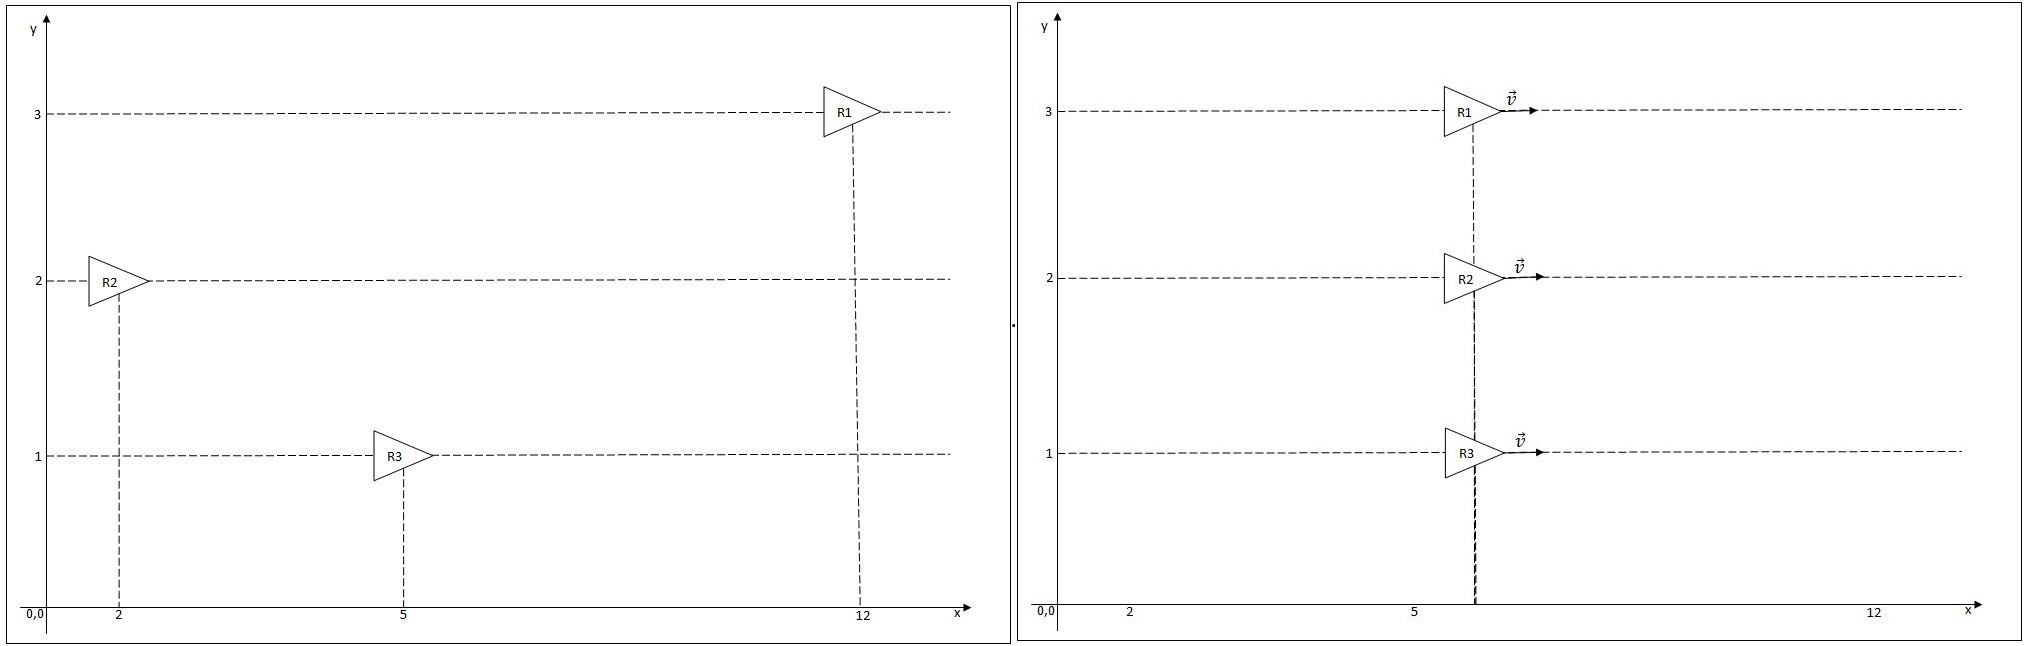
\includegraphics[width=16cm]{./04-figuras/p1}
	\caption{Problema 1: Fig.(a): Sistema no instante i. Fig.(b): Sistema no instante i+k.}
	\label{fig:p1}
\end{figure}

Supondo uma tropa de três robôs, orientados todos no mesmo sentido do eixo x, as velocidades de cada robô devem variar de acordo com o erro de posicionamento do mesmo no eixo x, conforme a distância entre os robôs. Conforme mostrado nas  equações \ref{eq:vel1P1}, \ref{eq:vel2P1} e \ref{eq:vel3P1}. Essas equações fazem com que o robô mais adiantado da frota, imprima uma velocidade menor que os outros robôs, tendendo a se aproximar dos mesmos, em contrapartida os robôs que estão "atrasados" imprimem uma velocidade maior, até que o erro entre eles seja zero e os mesmos caminhem com velocidade constante. 

\begin{equation}
v_{Robo1} = v_{d} + k \times erro_{2,1}
\label{eq:vel1P1}
\end{equation}
\begin{equation}
v_{Robo2} = v_{d} + k\times (erro_{1,2} + erro_{3,2})
\label{eq:vel2P1}
\end{equation}
\begin{equation}
v_{Robo3} = v_{d} + k\times erro_{1,3}
\label{eq:vel3P1}
\end{equation}

Onde,
\begin{itemize}
	\item $v_{Robo1}$, $v_{Robo2}$ e $v_{Robo3}$ são as velocidades que cada robô deve possuir para assumir a formação \emph{in line};
	\item $v_{d}$ é a velocidade que a frota deve assumir após estar alinhada;
	\item $k$ é a constante de ganho proporcional do controlador;
	\item E as variáveis de erro são calculadas, obtendo se a diferença entre a posição no eixo $x$ entre os robôs, como demonstrado na \autoref{eq:errp1}.	
\end{itemize}

\begin{equation}
erro_{i,j} = x_{i} - x_{j}
\label{eq:errp1}
\end{equation}

É importante notar que ao abordar o problemas desta maneira elimina-se o problema de colisão entre os robôs, que estão inicialmente separados no eixo y e alinhados no mesmo sentido, e assim seguem, visto que os mesmos não imprimem velocidade angular. Desta forma, tornando o problema bem didático para ser abordado inicialmente. Posteriormente, será mostrado o problema sendo abordado de outra forma.

\section{Problema 2: Rodeando um alvo}

%O segundo problema consistem em dado um alvo de posiçao $(x,y)$ no plano, a frota deve se locomover até o alvo e o circular, mantendo uma distância $R$ do alvo, com determinada velocidade angular que deve variar de acordo com o tamanho da frota.  

O segundo problema consiste em guiar uma frota de robôs a localizar e circundar, a uma distância \emph{R}, um alvo localizado em uma determinada posição (\emph{x,y}) do plano. E tem como objetivo secundário, ajustar a formação da tropa de robôs que deve se reajustar de acordo com o tamanho da frota, para que continue cobrindo com eficiência a fronteira. Ou seja, caso um ou mais robôs saiam da rede, a frota ira se reajustar para que cada robô tenha a mesma distância entre si e assim, não fique uma grande parte da fronteira sem cobertura, como demostrado na \autoref{fig:sistema}. Que representa uma frota de quatro robôs andando ao redor do alvo, quando então, um dos robôs falha. E o sistema se reajusta para adaptar-se à rede de apenas três robôs.

\begin{figure}[!htb]
	\centering
	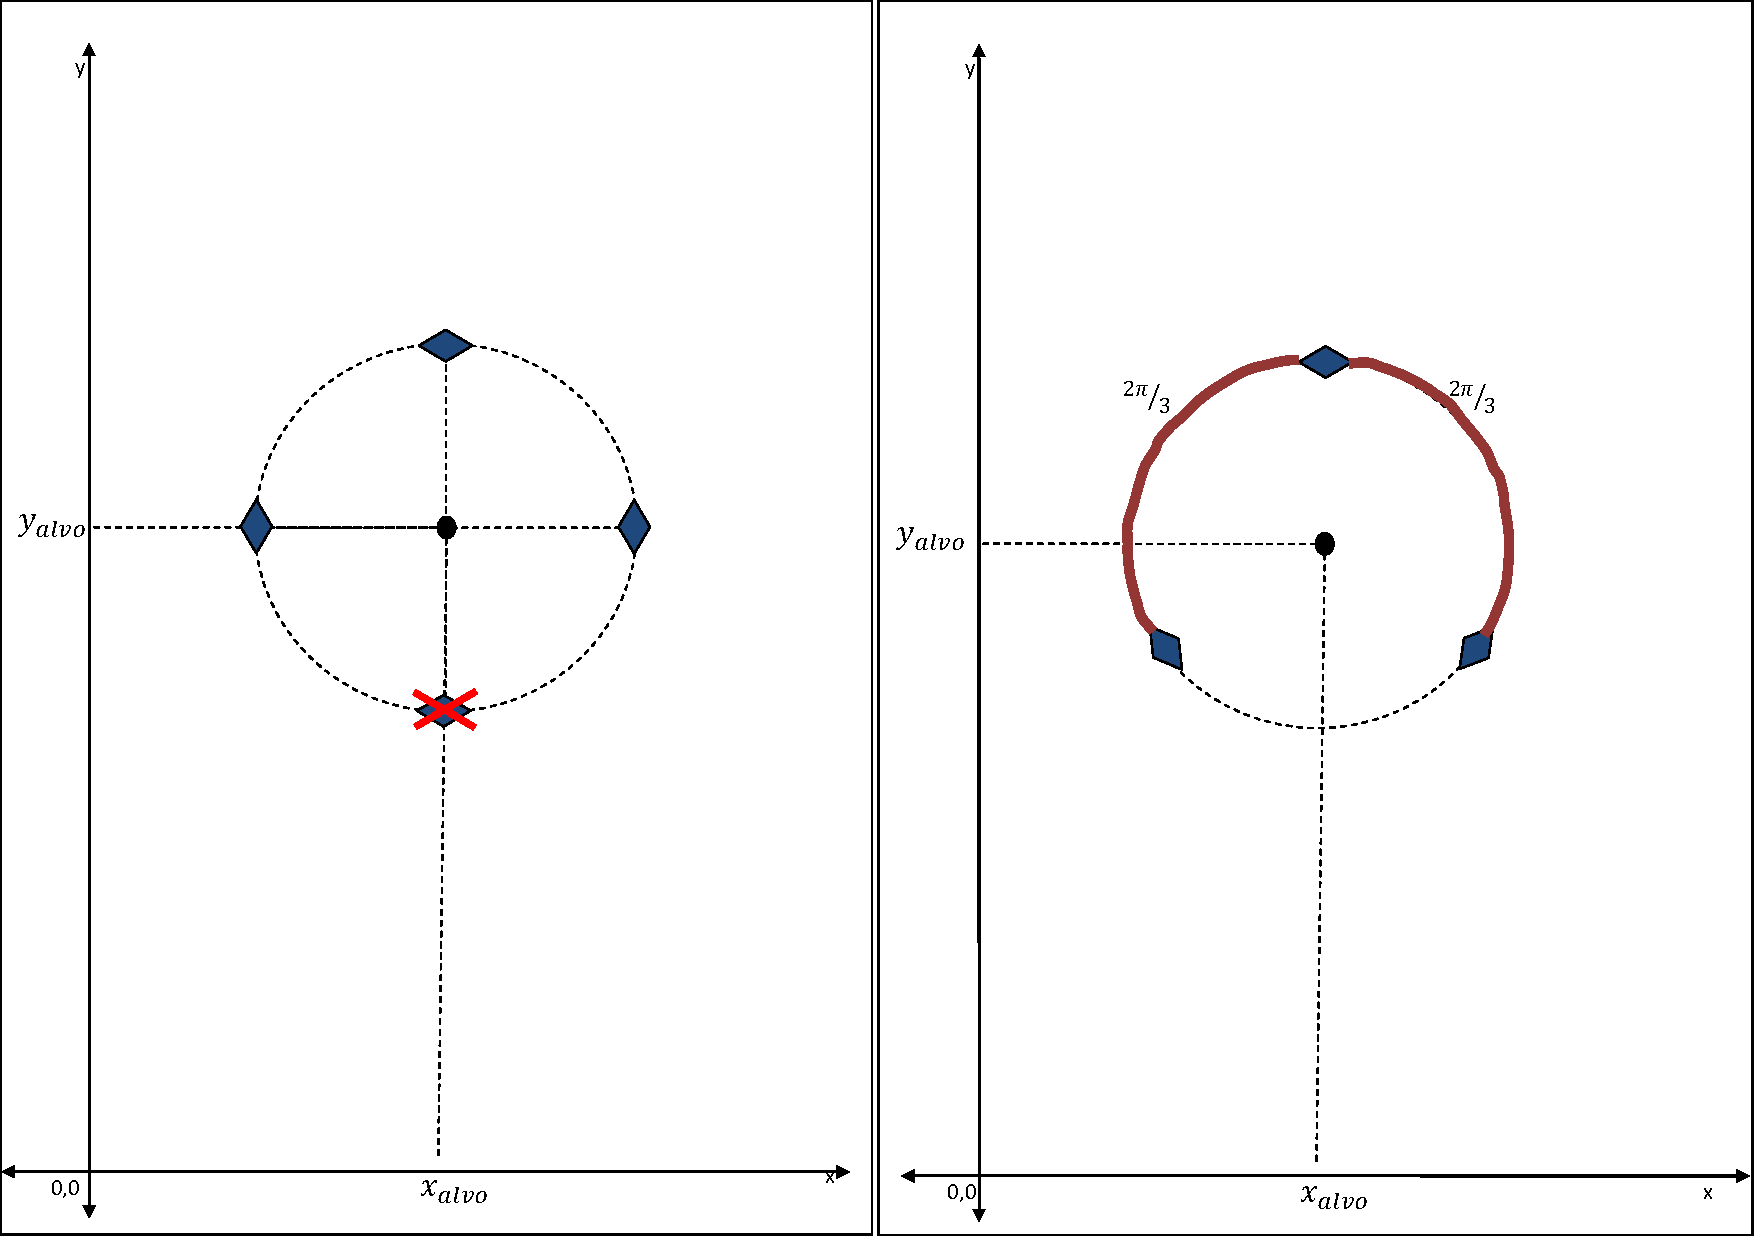
\includegraphics[width=1.0\textwidth]{./04-figuras/sistema}
	\caption{Modelagem do Sistema}
	\label{fig:sistema}
\end{figure}
